\documentclass[11pt,a4paper]{article}
\usepackage[utf8]{inputenc}
\usepackage[spanish]{babel}	%Idioma
\usepackage{amsmath}
\usepackage{amsfonts}
\usepackage{amssymb}
\usepackage{graphicx} 	%Añadir imágenes
\usepackage{geometry}	%Ajustar márgenes
\usepackage[export]{adjustbox}[2011/08/13]
\usepackage{float}
\restylefloat{table}
\usepackage[hidelinks]{hyperref}
\usepackage{titling}
\graphicspath{{/home/nazaret/Escritorio/LaTEX}}
%\usepackage{minted}
\usepackage{multirow}
\usepackage{caption}
\usepackage{multicol}
\usepackage[shortlabels]{enumitem}
\usepackage{array}
\selectlanguage{spanish}

%Opciones de encabezado y pie de página:
\usepackage{fancyhdr}
\pagestyle{fancy}
\lhead{Nazaret Román Guerrero}
\rhead{Redes Multiservicio}
\lfoot{Grado en Ingeniería Informática}
\cfoot{}
\rfoot{\thepage}
\renewcommand{\headrulewidth}{0.4pt}
\renewcommand{\footrulewidth}{0.4pt}

%Opciones de fuente:
\usepackage[utf8]{inputenc}
\usepackage[default]{sourcesanspro}
\usepackage{sourcecodepro}
\usepackage[T1]{fontenc}

\setlength{\parindent}{15pt}
\setlength{\headheight}{15pt}
\setlength{\voffset}{10mm}

% Custom colors
\usepackage{color}
\definecolor{deepblue}{rgb}{0,0,0.5}
\definecolor{deepred}{rgb}{0.6,0,0}
\definecolor{deepgreen}{rgb}{0,0.5,0}

\usepackage{listings}

\begin{document}
\begin{titlepage}

\begin{minipage}{\textwidth}

\centering

\includegraphics[width=0.5\textwidth]{img/logo.png}\\

\textsc{\Large Redes Multiservicio\\[0.2cm]}
\textsc{GRADO EN INGENIERÍA INFORMÁTICA}\\[1cm]

{\Huge\bfseries Valor de R para un códec\\}
\noindent\rule[-1ex]{\textwidth}{3pt}\\[3.5ex]
{\large\bfseries Seminario 1}
\end{minipage}

\vspace{1.5cm}
\begin{minipage}{\textwidth}
\centering

\textbf{Autora}\\ {Nazaret Román Guerrero}\\[2.5ex]

\includegraphics[width=0.3\textwidth]{img/etsiit.jpeg}\\[0.1cm]
\vspace{1cm}
\textsc{Escuela Técnica Superior de Ingenierías Informática y de Telecomunicación}\\
\vspace{1cm}
\textsc{Curso 2018-2019}
\end{minipage}
\end{titlepage}

\pagenumbering{gobble}
\pagenumbering{arabic}

\newpage

\begin{enumerate}
	\item \textbf{Representar la dependencia del valor $R$ con la probabilidad de pérdida de un paquete para un códec determinado.}
\end{enumerate}

El valor de $R$ proviene de la forma de medir del método E-model que proporciona una predicción de la calidad de voz según la siguiente fórmula:

\[R=R_0-l_s-l_d-le_eff+A\]

donde:

\begin{itemize}
	\item $R_0$ indica la relación señal-ruido.
	\item $l_s$, también llamado factor de simultaneidad, que indica los impedimentos que se dan simultáneos con la voz.
	\item $l_d$, también llamado factor de retardo.
	\item $le_eff$, también llamado factor de equipamiento, que indica las distorsiones producidad por el algoritmo de codificación y decodificación de la voz y por la pérdida de paquetes.
	\item $A$, también llamado factor de expectación, que indica el factor utilizado para modelar las deficiencias soportadas por los usuarios.
\end{itemize}

Teniendo esto en cuenta, vamos a hacer una comparativa con dos códecs diferentes, para ver el valor de $R$ en cada caso según el porcentaje de pérdida de paquetes. Para ello, vamos a utilizar una \color{blue}\href{https://www.voiptroubleshooter.com/diagnosis/emodel.html}{calculadora online} \color{black}del valor de $R$, donde podemos especificar el códec y el porcentaje de pérdida de paquetes y nos calculará el valor correspondiente.

\begin{enumerate}
	\item Códec: G.711 sin enmascarado de pérdida de paquetes, es decir, no se utiliza un algoritmo que oculte o disminuya el efecto de la pérdida.
	
	\begin{table}[H]
	\centering
		\begin{tabular}{|c|c|}
		\hline
		\textbf{\% de paquetes perdidos} & \textbf{Valor de R} \\ \hline
			0                                & 93                  \\ \hline
			2                                & 77                  \\ \hline
			5                                & 62                  \\ \hline
			10                               & 46                  \\ \hline
			15                               & 36                  \\ \hline
			20                               & 30                  \\ \hline
			25                               & 25                  \\ \hline
			30                               & 22                  \\ \hline
			40                               & 17                  \\ \hline
			50                               & 14                  \\ \hline
		\end{tabular}
	\caption{Comparativa entre el valor de $R$ y el porcentaje de paquetes perdidos. \textbf{Códec G.711}}
	\end{table}

Como se puede observar en el gráfico siguiente, claramente a mayor pérdida de paquetes peor es la estimación de la calidad de la voz:

	\begin{figure}[H]
	\centering
		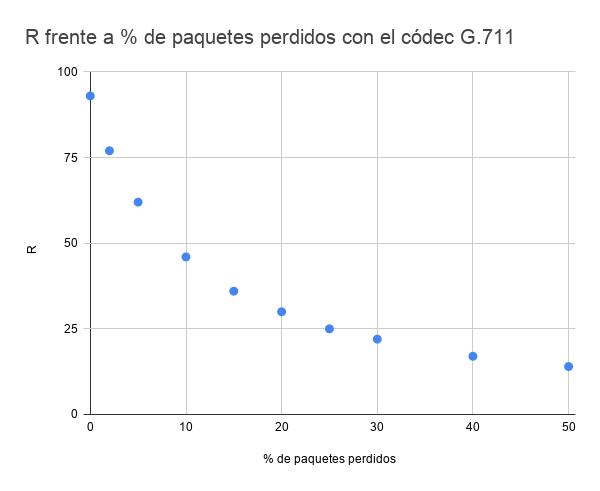
\includegraphics[scale=0.5]{img/grafico.png}
	\end{figure}
	
	\item Códec: iBLC 13k, un códec de banda estrecha.
	
	\begin{table}[H]
	\centering
		\begin{tabular}{|c|c|}
		\hline
		\textbf{\% de paquetes perdidos} & \textbf{Valor de R} \\ \hline
			0                                & 83                  \\ \hline
			2                                & 78                  \\ \hline
			5                                & 70                  \\ \hline
			10                               & 61                  \\ \hline
			15                               & 54                  \\ \hline
			20                               & 48                  \\ \hline
			25                               & 43                  \\ \hline
			30                               & 39                  \\ \hline
			40                               & 33                  \\ \hline
			50                               & 29                  \\ \hline
		\end{tabular}
	\caption{Comparativa entre el valor de $R$ y el porcentaje de paquetes perdidos. \textbf{iBLC 13k}}
	\end{table}
	
De nuevo, mirando el gráfico podemos ver que la calidad estimada es peor cuantas más pérdidas de paquetes se estimen. No obstante, este códec ofrece unos mejores resultados que el códec anterior:

	\begin{figure}[H]
	\centering
		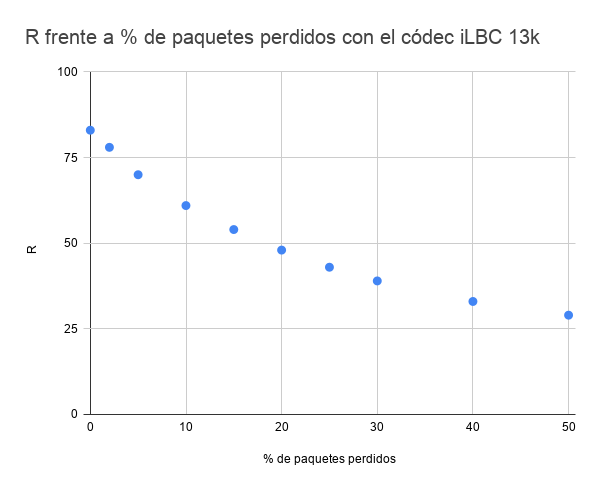
\includegraphics[scale=0.5]{img/grafico2.png}
	\end{figure}

\end{enumerate}

\end{document}